\chapter{Force analysis}

This chapter aims to analyse the findings presented in the previous two chapters, focusing on the intricate details and implications of Atomic Force Microscopy (AFM) force curve analysis. The preceding chapters laid a foundational understanding of the colloidal interactions and the work involved to process the raw data into a usable format. This chapter instead will focus on using the previous chapters' data to draw conclusions about collodial systems. The force-distance profiles obtained from AFM are analysed, providing a direct and nuanced insight into the particle interactions at an individual level. The force curves, reflecting the precise nature of forces acting at the nanoscale, will be juxtaposed against the bulk property measurements to draw a more comprehensive picture of the colloidal dynamics. This analysis will not only validate but also potentially challenge and refine the conclusions drawn from the bulk measurements, offering a more holistic understanding of the colloidal systems under study. Through this integrative approach, we aim to bridge the gap between our microscopic observations and derive behaviour on the macro scale. This chapter takes the following format, firstly over viewing the approach data, then the retract data.

\section{Approach force curves}



The interaction forces in macroscale colloidal suspensions was calculated as $F∗$, derived from rheological data and zeta potential measurements. This parameter provides a context between macroscopic rheological behavior and microscopic inter-particle forces in the context of varying ionic strengths. The calculation of $F∗=2.5d2σ∗$ was based on the Derjaguin approximation, a theoretical framework interaction forces in systems where particles are significantly larger than the range of their interaction forces, as overviewed in chapter 1. The choice of $F∗$ as a reference for comparison against the $F0$ values calculated by the previous 2 chapters, this was driven by the desire to establish a correlation between bulk suspension properties and individual particle interactions. By varying the ionic strength, we observed significant changes in $F∗$, reflecting alterations in the colloidal interactions. These changes were then meticulously compared with the $F0$ values to validate our approach and to provide a understanding of the colloidal behavior under different electrostatic conditions. This comparative analysis not only reinforced the validity of using $F∗$ as a proxy for understanding colloidal forces but also underscored the interplay between bulk rheological properties and particle-level forces.

\begin{figure}[!tbph!!!]
  \centering
  \subfloat[Site 1 curves.]{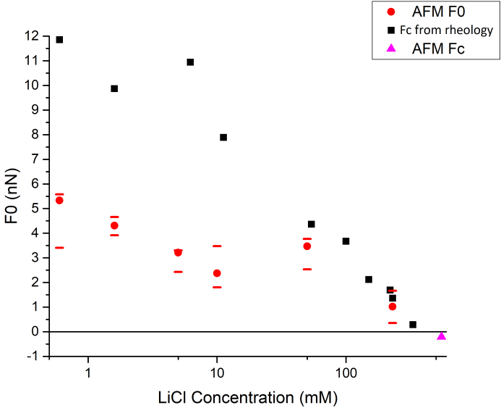
\includegraphics[width=0.45\textwidth]{chapter5/ContF1.png}\label{fig:CF1}}
  \hfill
  \subfloat[Site 2 curves.]{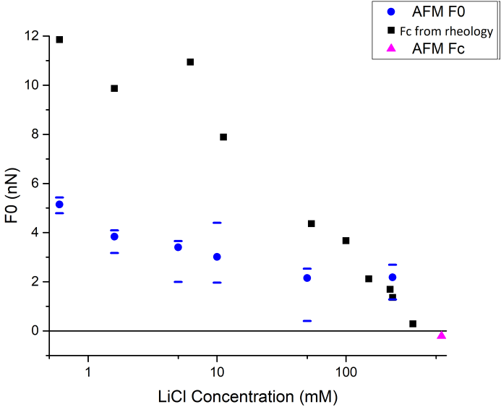
\includegraphics[width=0.45\textwidth]{chapter5/ContF2.png}\label{fig:CF2}}
  \caption{The resultant calculated repulsive force between the surface and the tip. The AFM data is compared against data taken from rheology. In the case of 550mM the repulsive forces transition to attractive, corresponding to the onset stress transitioning into yield stress (as seen from rheological data). F0 is taken from when the curve is within the onset of the contact region, Fc is taken from when the curve bends towards the surface, at the onset of contact (observable in \textit{Fig.3}. (a) and (b) are site 1 and 2 respectively\cite{John}.}
\end{figure}

\section{Shelf analysis}

The shelf seen in some datapoints 

\section{Variability in data}

The variability (noise) in the data may be due to the change in force applied to the surface. This is because the AFM is old and doesn't apply consistent pressure. It may have an affect, but you'd expect to see it more pronouced in the different salt concentrations. Plot the std dev vs concentration graph.

There is *alot* of noise at this scale. Because 
- I think it's cause it's a short period between phases?
- It's an old machine
- It hates me

Talk about how much noise there is. There is a lot of noise.

Show graphs

You can't just Lmao bin more cause then you have no data

\section{Lennard's potato}

\begin{equation} %Basic principles of colloid science
U_{rep} = \left(\frac{B}{a}\right) e^{-ar}
\end{equation}

Where $a$ and $B$ are constants. The Lennard-Jones potential is a result of these two equations, given by:

\begin{equation} %Basic principles of colloid science
U = U_{rep} + U_{att} = \left( \frac{B'}{r^{12}} \right) - \left( \frac{A'}{r^6}\right)
\end{equation}

%rewrite
Where $A'$ is a constant, related to the intrinsic quantum mechanical properties of the molecules in question.\cite{London}:

\begin{equation} %Basic principles of colloid science
A' = \left( \frac{3}{4} \right) h v \alpha^2
\end{equation}
%


%Consider Faraday's law - but only kinda. A_h = A' \pi^2 q^2
This expression describes $A'$ for two homogeneous molecules. $\alpha$ is the polarisability of the atom or molecule, $h$ is Plank's constant (6.63x10$^{-34}$ Js) and $v$ is the required frequency of a photon in order to ionise the molecule. In brief this equation describes the relationship between the van der Waals radius and the ionisation enthalpy, and thus encapsulates the interplay from the distance vs the size of the particles itself (as electron shell size increases, less energy is needed to ionise).
% CHECK: DO I USE h ELSEWHERE? /!\

\subsection{Electro Kabpapoorwpagka}
\begin{equation} %From foundations of collodial science. Why is it different than everywhere else I see it? (though this isn't quite right for our system) THIS IS FOR A VACUUM
\kappa = \left(\frac{e^2\Sigma n_{oi} z^2_i}{\epsilon k_B T}\right)^2 
\end{equation}

%Basic principles of collodial science
\begin{equation} 
\frac{1}{\kappa} = \left(\frac{\epsilon kT}{e^2 \Sigma c_i z_i^2}\right)^\frac{1}{2}
\end{equation}

%Basic principles of collodial science
\begin{equation} 
\frac{1}{\kappa} = \left(\frac{\epsilon RT}{F^2 \Sigma c_i z_i^2}\right)^\frac{1}{2}
\end{equation}
%F is faraday constant

%Intermolecular and surface forces
\begin{equation} 
\kappa = \left(\frac{e^2 \sum_{i} p_{\infty i} z_i^2} {\epsilon \epsilon_0 k T}  \right)^\frac{1}{2} 
\end{equation}\textbf{}

 F is Faraday's constant, $z_i$ is the valence of i ions
 
 %Old eqn simplified r/h to cancel each other out
\begin{equation} %This can't be right??
U_E (r) = 4\pi\epsilon \frac{R}{2 + \frac{h}{R}}\Psi^2_{0} e^{-\kappa r}
\end{equation}

%Replaced
\begin{equation} 
U_E (r) = \frac{2\pi h \sigma^2 e^{-\kappa}}{\kappa \epsilon \epsilon_0}
\end{equation}

%Simplified
\begin{equation} %This can't be right??
U_E (r) = 4\pi\epsilon \frac{R}{2}\Psi^2_{0} \epsilon_0 e^{-\kappa h}
\end{equation}

 $\approx \epsilon \epsilon_0 \kappa \Psi_0$
 
%Poission boltzman Debbie shuckle

This model was then revised under the Gouy-Chapman model in 1910-1913, \cite{34} which pays respect to the thermodynamic nature of the system. Which relies on the Poisson-Boltzmann equation.

\begin{equation} %possibly unneeded
\delta ^2 \Psi = \frac{\delta^2 \Psi}{\delta x^2} + \frac{\delta^2 \Psi}{\delta y^2} + \frac{\delta^2 \Psi}{\delta z^2} = - \frac{p_e}{\epsilon \epsilon_0}
\end{equation}

Debye-H\"uckle approximation linearises said Poisson-Boltzmann equation. In cases where $\Psi$ is small enough to approximate out, the Debye-H\"uckle parameter is given by: %We CANT assume Psi, it's a factor in our system.

\begin{equation} 
\kappa =  \sqrt{\frac{2000 F^2}{\epsilon \epsilon_0 R T}} \sqrt{I}
\end{equation}

$\kappa^-1$, the which is the characteristic Debye length of a system. However, in the case of colloids, Psi cannot nessicarily be assumed, and is given by  %It can but also it can't great (maybe calculate psi)
%why does psi need k when you need psi for k

 From this basis the Helmholtz model was born to consider the ionic radius. This ionic radius is used to understand the finite ionic adsorption. %Maybe remove - unnecessary detail?
 
\begin{equation}
\kappa = \sqrt{\frac{\epsilon_r \epsilon_0 k_b T}{2 N_A e^2 I}}
\end{equation}

Where $\epsilon_r$ is the dielectric constant which was taken from \cite{WaterGlycerolEpR}. $\epsilon_0$ is the absolute dielectric permittivity. $k_b$ is the Boltzmann constant, $N_A$ is Avogadro's constant,  $e$ is the charge, $I$ is ionic strength and $T$ is temperature.

\section{Effects of hydrodynamics}

\newpage.
\newpage

\section{Dwell time effects}

\newpage.
\newpage.
\newpage

\section{pH effects}

\newpage
\newpage

\section{Force mapping}


